%----------------------------------------------------------------------------------------
%	ANALISI DI DEPLOYMENT SU LARGA SCALA
%----------------------------------------------------------------------------------------

\section{Analisi di deployment su larga scala}
Il paradigma a microservizi da noi adottato si adatta perfettamente al deployment su larga scala.
Il progetto è stato fin da subito pensato per l'esecuzione in cloud, utilizzando appieno gli Amazon Web Services anche durante lo sviluppo locale.

Di seguito descriveremo in prima fase l'architettura adottata per il deployment, 
passeremo poi ad illustrare come viene praticamente eseguito il deployment sui vari ambienti (locale, staging e production), 
ed infine quali sono i costi totali del sistema. 

\subsection{Architettura Cloud}

Il progetto Ecotrip si basa sul raccogliere dati da una moltitudine di camere di una moltitudine di hotel, 
analizzarli ed aggregarli al fine di calcolare punteggi da fornire ad una moltitudine di utenti (visitatori e albergatori).

In prima battuta però Ecotrip verrà adottato da un singolo Hotel, è chiara quindi l'esigenza di un'architettura di deployment 
che consenta di partire con costi ridotti e che permetta una scalabilità orizzontale al bisogno.

Per ottenere questo abbiamo impiegato il paradigma Serverless per le componenti che richiedono una forte scalabilità, 
come il caricamento e lo stoccaggio dei dati, l'elaborazione e la fornitura verso gli utenti finali. 
Serverless significa impiegare servizi Cloud che scalano in automatico all'occorrenza, senza alcuna pianificazione prestabilita o intervento umano.

In Figura 22 mostriamo l'architettura implementata utilizzando diversi servizi messi a disposizione da Amazon Web Services (AWS).

Poiché questo è un progetto IoT, abbiamo scelto di utilizzare \textbf{DynamoDB}, il database serverless fornito da AWS, il quale è in grado di scalare automaticamente sia per quello che concerne la quantità di dati che per il numero di richieste al secondo.
Abbiamo suddiviso il database in tre tabelle: "IoTData" per i dati IoT inviati dalla Control Unit, "Administration" per la gestione della REST API, e "DataElaboration" per l'elaborazione dei dati. 
Questa suddivisione ci permette di gestire in modo efficiente e organizzato i dati del progetto, strutturando al meglio ogni tabella secondo le logiche di data modelling per un database NoSQL di tipo Key-Value.
Da notare che le entità di \textit{Administration} illustrate in fase progettuale sono confluite nella pratica in un'unica tabella DynamoDB: per arrivare a questo risultato abbiamo seguito le best-practices per il design di database NoSQL che richiede un approccio diverso dalla progettazione di RDBMS.

\begin{figure}[H]
    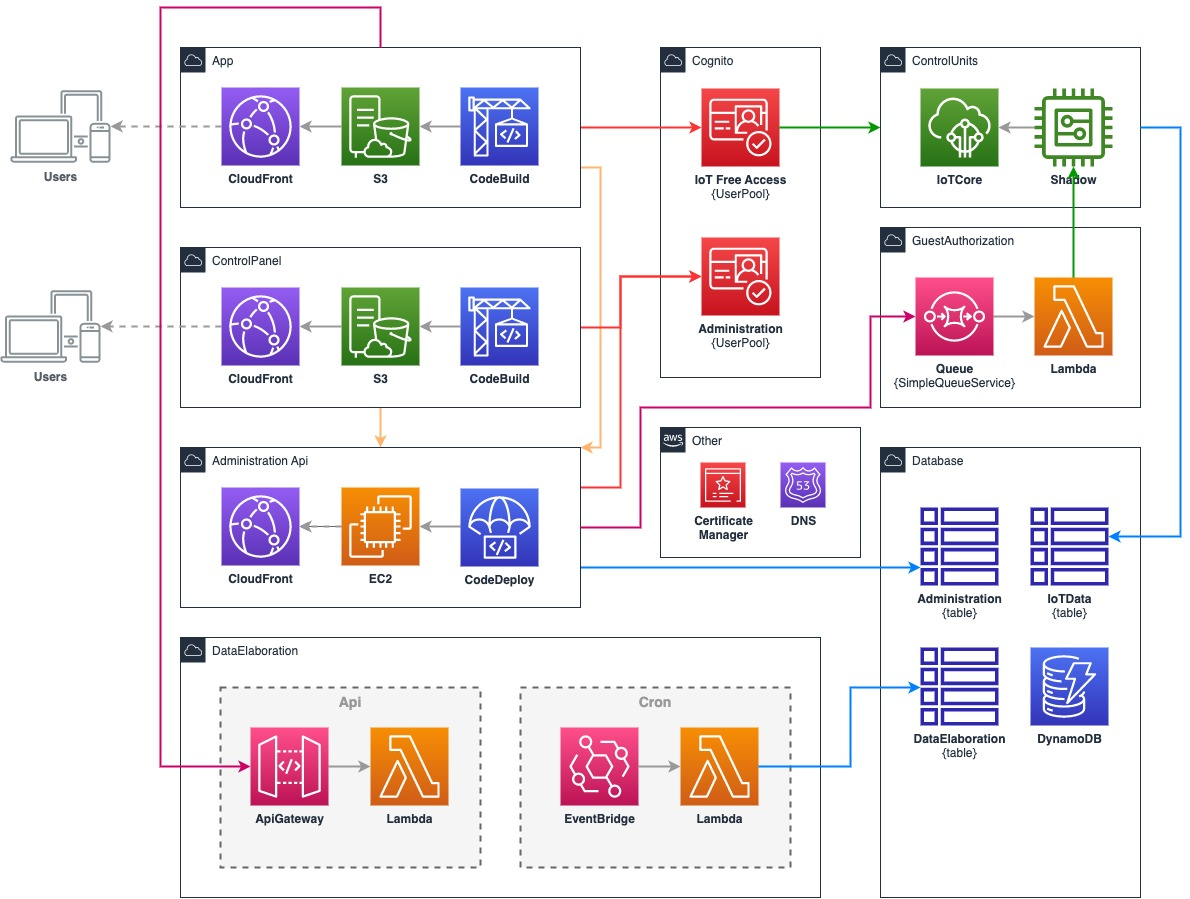
\includegraphics[width=\textwidth]{AWS.jpg}
    \centering
    \caption[aws]{Architettura AWS}
    \label{fig:aws}
\end{figure}

Il servizio \textbf{IoT Core} gestisce le centraline IoT e il loro stato attraverso la \textbf{copia shadow}. La copia shadow rappresenta una versione virtuale dello stato di ogni centralina IoT, che viene mantenuta sincronizzata con la centralina stessa. Inoltre si preoccupa di ricevere i dati delle centraline attraverso messaggi MQTT e stoccarli attraverso una opportuna regola sulla tabella IoTData.

La \textbf{REST API} della parte "Administration" è distribuita attraverso una istanza \textbf{EC2}.
Il traffico richiesto per questo componente è relativamente basso in quanto la API "Administration" è soprattutto utilizzata dal pannello di controllo, e si assume che vengano fatte richieste contemporanee da al massimo un utente per hotel, oltre ai visitatori che attraverso le app ricevono limitate informazioni sull'hotel (il nome) e il pernottamento corrente.
Per questo, in questa prima fase, si è scelto di non dotare il servizio API di scaling automatico tramite l'aggiunta di un load balancer.
In futuro la EC2 potrebbe essere sostituire da un servizio API Gateway che consente la completa scalabilità on demand tramite l'impiego di Lambda per ogni endpoint.

Le applicazioni single page (SPA) del pannello di controllo e web app sono distribuite tramite \textbf{CloudFront} di Amazon Web Services ed archiviate in un bucket S3. CloudFront è una rete di distribuzione dei contenuti (CDN) su server dislocati in tutto il mondo, il che garantisce una bassa latenza e una consegna veloce per gli utenti, indipendentemente dalla loro posizione geografica.

La generazione del token per i visitatori del microservizio "Guest Authorization" avviene su una \textbf{Lambda}, questa si attiva alla ricezione di un messaggio inviato da "Administration" attraverso il servizio di coda \textbf{Simple Queue Service} impostato in modalità FIFO (FirstIn-FirstOut). La Lambda si occuperà di aggiornare il valore del token sulla copia shadow del dispositivo fisico, dopo averlo ricercato all'interno del servizio IoT Core attraverso attributi univoci che identificano la centralina di una determinata stanza di un albergo.

Per l'elaborazione dei dati da parte di "Data Elaboration" è stata impiegata un'altra Lambda che si attiva periodicamente ogni 5 minuti attraverso un'attività pianificata di tipo \textbf{EventBridge}. Dopo aver eseguito i calcoli questi vengono memorizzati su un apposta tabella "DataElaboration" in DynamoDB.
Attualmente i dati da elaborare vengono processati da un unica istanza della Lambda, ma è possibile strutturare il sistema in modo che ogni hotel avvii la sua istanza di Lambda periodicamente per processare unicamente i suoi dati: questo consente la totale scalabilità computazionale anche per quanto riguarda questo servizio che è il più critico ed oneroso in termini di costo di CPU.
La fornitura dei dati elaborati, come i consumi di un pernottamento o il punteggio sostenibilità richiesti dai visitatori o albergatori, avviene attraverso una REST API realizzata con \textbf{API Gateway}: servizio di Amazon che permette ad una API di abbracciare in pieno il paradigma Serverless e quindi piena scalabilità on-demand.

Per quanto riguarda la gestione degli utenti, abbiamo utilizzato \textbf{Cognito}. Abbiamo creato due diverse pool di utenti: una per il pannello di controllo "Administration" e un'altra per gli accessi liberi "IoT Free Access". La pool di utenti "Administration" fornisce l'accesso al pannello di controllo per gestire la configurazione e gestione degli alberghi, stanze e prenotazioni. La pool di utenti "IoT Free Access", d'altra parte, consente agli utenti sull'App di visualizzare i dati MQTT in tempo reale della parte IoT senza la necessità di una registrazione.
Cognito emette un token di autorizzazione per ogni sessione di accesso degli utenti, che può essere utilizzato per autorizzare le richieste API. Il token di autorizzazione scade dopo un certo periodo di tempo, ma gli utenti possono ottenere un nuovo token di autorizzazione tramite il token di refresh. Questo sistema a due token garantisce la sicurezza dei dati degli utenti e delle applicazioni, poiché i token di autorizzazione possono essere revocati o scadere in qualsiasi momento, senza che ciò influisca sulla sessione di accesso degli utenti. 

\subsection{Ambienti di deployment}

Il deployment è un aspetto cruciale per questo tipo di progetto, per questo ci siamo concentrati subito sul definire come lavorare e sviluppare in locale con i servizi cloud.

Abbiamo predisposto 3 ambienti: \textbf{locale}, \textbf{staging} e \textbf{production}.

Per quanto riguarda lo sviluppo in locale, abbiamo creato un ambiente che riproduce l'architettura descritta in precedenza. 
Utilizzando \textbf{Docker Compose}, abbiamo emulato le due Applicazioni (App e ControlPanel), la REST API e il database DynamoDB in container separati. Mentre per quanto riguarda i servizi rimanenti (Cognito, DataElaboration e GuestAutorizzazione) abbiamo utilizzato script che compilano ed avviano template in \textbf{SAM} per creare stack in \textbf{CloudFormation}, effettuando così il deploy direttamente su AWS dei servizi per il singolo componente del team. 
In questo modo il team di sviluppo può lavorare sul progetto in modo semplice e rapido. Tutto ciò che serve è scaricare il repository che include tutti i sotto-moduli necessari. Con un semplice script, l'ambiente locale viene preparato utilizzando Docker Compose e la parte online su AWS viene avviata attraverso stack di CloudFormation. Questo processo viene effettuato in modo specifico per ogni singolo membro del team, garantendo così un ambiente di sviluppo personalizzato e indipendente.

SAM (\textbf{Serverless Application Model}) è un framework opensource che attraverso modelli permette di descrivere l'architettura cloud da creare e gestire. SAM è stato progettato per semplificare la creazione e la gestione di applicazioni serverless utilizzando CloudFormation, senza dover accedere manualmente alle interfacce di gestione di AWS.

In fase di staging e production, il processo di deployment viene completamente automatizzato tramite le \textbf{GitHub Action} sulle apposite branch. Queste azioni avviano i relativi script che attraverso i template SAM creano e mantengono aggiornata l'infrastruttura su AWS, garantendo così un processo di distribuzione affidabile, efficiente e privo di errori. Il sistema di deploy automatico garantisce che il progetto sia sempre allineato alla versione più recente.

L'ambiente di staging è una replica fedele dell'ambiente di produzione, che viene utilizzato per effettuare test e verifiche prima di effettuare eventuali modifiche al sistema in produzione. Questo ambiente separato permette di effettuare prove senza influire sul funzionamento e sui dati del sistema in produzione, garantendo così la stabilità e la sicurezza dell'intero ecosistema.

\newpage